\documentclass[12pt]{article}
\usepackage[12pt]{moresize}
\usepackage[margin=1in]{geometry}

\usepackage{amsmath}
\usepackage{amssymb}

\usepackage{graphicx}
\usepackage{subcaption}

\usepackage{multirow} %Combining rows in tables
\usepackage{diagbox}  %Table box split in twain
\usepackage{hhline}
\usepackage{makecell} 

\usepackage[ruled,linesnumbered]{algorithm2e}
\usepackage{algpseudocode}
\usepackage{alltt}

\usepackage{multicol}

\usepackage{amssymb} %\checkmark symbol

%\usepackage{hyperref}
%\usepackage[latin1]{inputenc}
%\usepackage{listings}
%\usepackage{scrextend}
%\usepackage{changepage} %Adjustwidth

 

\title{ComS 474\\Homework 7}
\author{Sean Gordon}
\date{Nov 20, 2020}

\begin{document}
\maketitle


\section{K-means}


\noindent 1) $X_i \in cluster1$\ \ if\ \ $dist(X_i, C_1) < dist(X_i, C_2)$, meaning $||X_i - C_1||^2 < ||X_i - C_2||^2$,\\
\indent else $X_i \in cluster2$\\\\\\


\noindent 2) Step 1: For a point $x$, calculate the euclidean distance $d_i$ to each centroid $C_i$.\\
\indent Step 2: Select the smallest $d_i$ and record the index $i$.\\
\indent Step 3: Assign x to the cluster of the respective centroid $C_i$.\\
\indent Step 4: Repeat steps 1-3 for all points in X.\\

\indent Using the steps above, it can be found that each cluster contains the points below:\\
\indent Cluster 1: [0, 4, 5], Cluster 2: [1, 2, 3]\\

\indent These values were calculated using the \textproc{closest(x, C)} function in kmeans.py.\\\\\\


\noindent 3) Step 1: For a centroid $C$, calculate the arithmetic mean $M$ for all points in its cluster.\\
\indent Step 2: Assign $C$ the calculated value $M$.\\
\indent Step 3: Repeat this for all centroids C.\\

\indent $C_1$ = {\Large $\frac{(-0.57, 0.87, -0.89)+(-0.28, 0.25, -1.54)+(-1.18, 1.26, -0.33)}{3}$} $\Rightarrow$ \\
\indent $C_1$ = (-0.6767, 0.7933, -0.92)\\

\indent $C_1$ = {\Large $\frac{(0.04, -0.76, 0.41)+(0.55, -0.38, 0.56)+(-0.65, -1.66, 0.35)}{3}$} $\Rightarrow$ \\
\indent $C_1$ = (-0.02, -0.9333, 0.44)\\



\noindent \hrulefill \\\pagebreak


\section{Single-linkage clustering}\ \\


\noindent 4) 
\begin{tabular}{ccccccc}
\hhline{-------}\\[-1em]
 & (1) & (2) & (3) & (4) & (5) & (6)\\[.2em]
\hhline{-------}\\[-1em]
(1) & 0 & 2.17232594 & 2.21797205 & 2.8186699  & 0.94392796 & 0.91531415 \\
(2) & 2.17232594 & 0 & 0.65345237 & 1.13564959 & 2.2192341  & 2.47313566 \\
(3) & 2.21797205 & 0.65345237 & 0 & 1.7670597 & 2.34431227 & 2.54452353 \\
(4) & 2.8186699 & 1.13564959 & 1.7670597 & 0 & 2.71239746 & 3.0446182 \\
(5) & 0.94392796 & 2.2192341 & 2.34431227 & 2.71239746 & 0 & 1.81499311\\
(6) & 0.91531415 & 2.47313566 & 2.54452353 & 3.0446182 & 1.81499311 & 0\\
\hhline{-------}
\end{tabular}\\\\



\noindent 5) As clusters 2 and 3 have the shortest distance between them (0.6534), they should be\\
\indent merged.\\



\noindent 6) 
\begin{tabular}{ccccccc}
\hhline{-------}\\[-1em]
 & (1) & (2) & (3) & (4) & (5) & (6)\\[.2em]
\hhline{-------}\\[-1em]
(1) & 0 & 2.17232594 & 2.21797205 & 2.8186699  & 0.94392796 & 0.91531415 \\
(2) & 2.17232594 & 0 & \textbf{0.65345237} & 1.13564959 & 2.2192341  & 2.47313566 \\
(3) & 2.21797205 & \textbf{0.65345237} & 0 & 1.7670597 & 2.34431227 & 2.54452353 \\
(4) & 2.8186699 & 1.13564959 & 1.7670597 & 0 & 2.71239746 & 3.0446182 \\
(5) & 0.94392796 & 2.2192341 & 2.34431227 & 2.71239746 & 0 & 1.81499311\\
(6) & 0.91531415 & 2.47313566 & 2.54452353 & 3.0446182 & 1.81499311 & 0\\
\hhline{-------}
\end{tabular}\\\\

\begin{tabular}{cccccc}
\hhline{------}\\[-1em]
 & (1) & (2, 3) & (4) & (5) & (6)\\[.2em]
\hhline{------}\\[-1em]
(1) & 0 & 2.17232594 & 2.8186699  & 0.94392796 & \textbf{0.91531415} \\
(2, 3) & 2.17232594 & 0 & 1.13564959 & 2.2192341  & 2.47313566 \\
(4) & 2.8186699 & 1.13564959 & 0 & 2.71239746 & 3.0446182 \\
(5) & 0.94392796 & 2.2192341 & 2.71239746 & 0 & 1.81499311\\
(6) & \textbf{0.91531415} & 2.47313566 & 3.0446182 & 1.81499311 & 0\\
\hhline{------}
\end{tabular}\\\\

\begin{tabular}{ccccc}
\hhline{-----}\\[-1em]
 & (1, 6) & (2, 3) & (4) & (5)\\[.2em]
\hhline{-----}\\[-1em]
(1, 6) & 0 & 2.17232594 & 2.8186699  & \textbf{0.94392796}\\
(2, 3) & 2.17232594 & 0 & 1.13564959 & 2.2192341\\
(4) & 2.8186699 & 1.13564959 & 0 & 2.71239746\\
(5) & \textbf{0.94392796} & 2.2192341 & 2.71239746 & 0\\
\hhline{-----}
\end{tabular}\\\\

\begin{tabular}{cccc}
\hhline{----}\\[-1em]
 & (1, 5, 6) & (2, 3) & (4)\\[.2em]
\hhline{----}\\[-1em]
(1, 6) & 0 & 2.17232594 & 2.71239746  \\
(2, 3) & 2.17232594 & 0 & 1.13564959 \\
(4) & 2.71239746 & 1.13564959 & 0 \\
\hhline{----}
\end{tabular}\\\\\pagebreak

\begin{center}Dendrogram:\end{center}
\begin{figure}[h!]
  \centering
  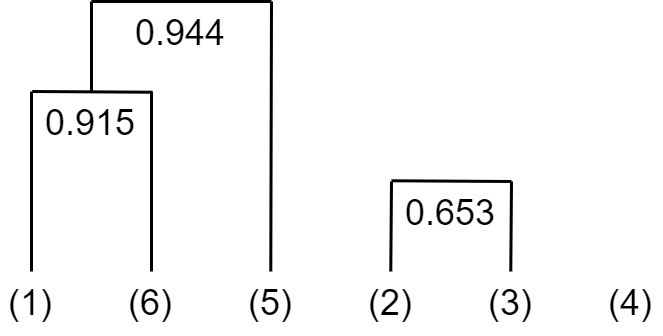
\includegraphics[scale=.5]{Pics/Q6.png}
\end{figure}




\noindent \hrulefill \\\pagebreak



\section{DBSCAN}\ \\


\noindent 7) Neighbors = \{B, C, D, G\}.\\\\


\noindent 8) A sample is a core point if its number of neighbors $>$ T.\\[.4em]
\indent B has 1 neighbor A. \ \ C has 3 neighbors A, E, F. \\
\indent D has 1 neighbor A. \ \ G has 4 neighbors A, H, I, J.\\[.4em]
\indent As the only neighbor of A that has $>$ 3 neigbors is G, G is the only neigbor of A \\
\indent that is a core point.\\


\begin{multicols}{2}

\noindent 9) \ C=\{A\}\\
\indent C=\{A,B,C,D,G\}\\
\indent C=\{A,B,C,D,G,H,I,J\}\\
\indent C=\{A,B,C,D,G,H,I,J,K\}\\
\indent C=\{A,B,C,D,G,H,I,J,K,L,N\}\\

\columnbreak

\ \\
Added from A\\
Added from G\\
Added from I\\
Added from K\\

\end{multicols}


\noindent 10)\begin{algorithm}
\caption{Shortened DBSCAN Pseudocode.}
\BlankLine
\KwData{$X$: samples, $T$:, a threshold}
\BlankLine
\BlankLine
Initialize cluster index i $\leftarrow$ 1\;
\ForEach{sample $x$ $\in$ $X$}{
	\If{$x$ are NOT assigned to a cluster}{
		\BlankLine
		Seed set of cluster $i$: $S$ $\leftarrow$ $x$\;
		\BlankLine
		\While{$S$ $\neq$ $\emptyset$}{
			$y$ $\leftarrow$ one element of $S$\;
			\If{$|$N(y)$|$ $>$ T}{
				Assign $y$ to cluster $i$\;
				$S$ $\leftarrow$ $S$ $\cup$ $N(y)$\;
			}
			\BlankLine
			Remove $y$ from $S$\;
		}
	\BlankLine
	i++\;
	}
}
\end{algorithm}





%\begin{figure}[htbp]
%\centerline{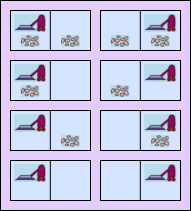
\includegraphics{Pics/ComS472_410.png}}
%\caption{Belief states recheable from initial 8 belief states.}
%\label{Belief states recheable from initial 8 belief states.}
%\end{figure}

\end{document}

















